


\section{Related Work}
\subsection{Deepfakes generation}
The recent advances in deep generative models significantly im-
prove face manipulation techniques, such as GAN face synthesis
, facial attribution editing face swapping  and etc.
In particular, one technique known as DeepFake attracts tremen-
dous attention. DeepFake is a face swapping technique that can
swap the source face of input image with a synthesized target face
while keeping the same facial expression and orientation. Specifi-
cally, DeepFake is based on variational auto-encoder (VAE) archi-
tecture , where the encoder aims to remove identity-related
attributes and the decoder aims to recover the appearance of tar-
get identity. The overview of DeepFake video generation is shown
in Fig. 1. 
\vspace{1cm}

\begin{figure}[h]
    \centering
    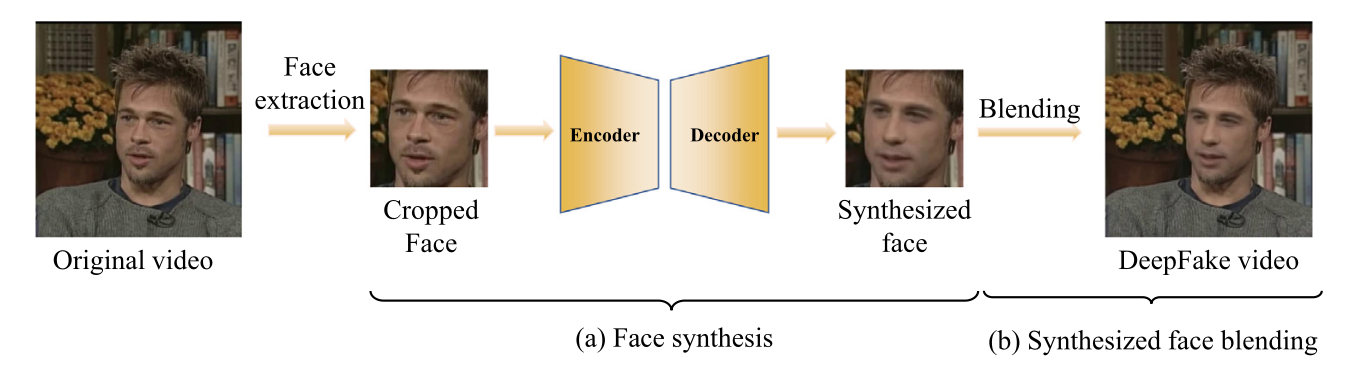
\includegraphics[width=1\textwidth]{figures/fig1.png}
    \caption{Deepfake Generation}
    \label{fig:enter-label}
\end{figure}


\subsection{Deepfakes detection}
Many DeepFake detection methods have been proposed so far,
e.g.,  We divide these methods into four categories: data-
driven, frequency based, artifacts based and consistency based. The
data-driven denotes training detector directly using real and Deep-
Fake images. For example, MesoNet , XceptionNet  and Cap-
suleNet , which trained their advised networks using real and DeepFake images. MTD-Net  proposed Central Difference Con-
volution (CDC) and Atrous Spatial Pyramid Pooling (ASPP) to fur-
ther improve the performance. For frequency based methods, Agar-
wal et al.  proposed a novel cross-stitched network to mine the
distinguishing features in the spatial and frequency domains. Luo
et al. employed the SRM filters to extract the high-frequency
noise feature, and proposed a multi-scale high-frequency feature
extraction module to capture multi-scale high-frequency signals.


